
%403
\section{Determinantes}


\subsection{Tipos de sistemas}
\begin{figure}
	\centering
	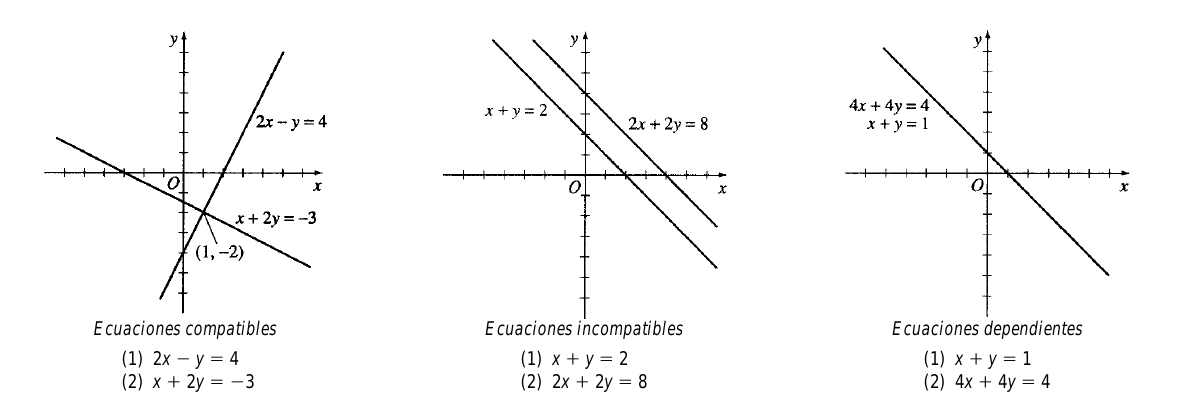
\includegraphics[width=12cm,keepaspectratio=true]{./precalculo/IM0402.png}
	% IM0402.png: 0x0 pixel, 300dpi, 0.00x0.00 cm, bb=
	\label{fig:0401}
\end{figure}

\subsection{Determinantes de Segundo Orden}

	\begin{definicion}
		$$
		\begin{vmatrix}
			a & b \\ c & d
		\end{vmatrix}=ad-bc.
		$$
	\end{definicion}




	\begin{resuelto}
		Calcula el siguiente determinante
		$$
		\begin{vmatrix} 2 & 3 \\ -1 & -2 \end{vmatrix}
		$$
	\end{resuelto}



\subsection{Método de Cramer}

	Si consideremos el siguiente sistema de ecuaciones
	\[
		\begin{cases}
			a_{1}x+b_{1}y=c_{1}\\
			a_{2}x+b_{2}y=c_{2}
		\end{cases}
	\]
	y definimos
	\begin{align*}
		\Delta&=\begin{vmatrix} a_{1} & b_{1} \\ a_{2} & b_{2} \end{vmatrix}\\
		\Delta_{x}&=\begin{vmatrix} c_{1} & b_{1} \\ c_{2} & b_{2} \end{vmatrix}\\
		\Delta_{y}&=\begin{vmatrix} a_{1} & c_{1} \\ a_{2} & c_{2} \end{vmatrix}
	\end{align*}
	entonces
	\[
		\label{spi:28.2}
		\begin{split}
			x&=\dfrac{\Delta_{x}}{\Delta}\\
			y&=\dfrac{\Delta_{y}}{\Delta}
		\end{split}
	\]




	\begin{resuelto}
		Resuelva el sistema
		$$\begin{cases}
			2x+3y=8\\
			x-2y=-3
		\end{cases}
		$$
	\end{resuelto}





\subsection{Sistemas Indeterminados}


	Un sistema de $ n $ ecuaciones con $ n $ incognitas tiene una única solución si y solo si su determinante principal $ \Delta \neq 0. $

	En este caso, decimos que el sistema es consistente.



	Si $ \Delta =0 $, entonces o bien existen multiples soluciones, o bien no existe alguna en absoluto.

	En cualquier caso, decimos que el sistema es inconsistente.



	Determine si
	$$\begin{cases}
		5x-2y=10\\
		10x-4y=20
	\end{cases}$$
	es consistente; y de no ser el caso, explique que sucede con las soluciones.



	Determine si
	$$\begin{cases}
		5x+3y=15\\
		10x+6y=60
	\end{cases}$$
	es consistente; y de no ser el caso, explique que sucede con las soluciones.






